% !TeX spellcheck = cs_CZ
\begin{example}\label{TEO:ex_NeinvOpamp01} 
  Uvažujme neinvertující zesilovač s ideální operačním zesilovačem typu VFA s naznačenými uzly tak, 
  jak je na obr. \ref{TEO:fig_MMUN_neinv_opamp}. Napište rovnice MMUN.

   {\centering
    \captionsetup{type=figure}
    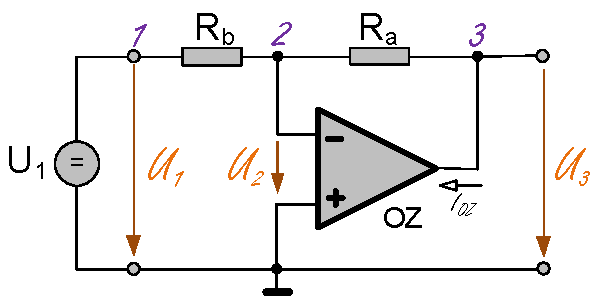
\includegraphics[width=0.7\linewidth]{MMUN_inv_OPAMP.pdf}
    \captionof{figure}{Neinvertující zesilovač}
    \label{TEO:fig_MMUN_neinv_opamp}
    \par}
   % using \usepackage{array} and command \newcolumntype{C}[1]{>{\centering}m{#1}}!
  {\centering
   \begin{tabular}{|C{0.45cm}|C{1.2cm}|C{0.6cm}|C{0.45cm}|C{0.45cm}|C{0.2cm}|c|C{.3cm}|c|}
      \multicolumn{1}{c}{$U_1$} & \multicolumn{1}{c}{$U_2$}   & \multicolumn{1}{c}{$U_3$} & 
      \multicolumn{1}{c}{$I_1$} & \multicolumn{1}{c}{$I_{OZ}$}& \multicolumn{1}{c}{ }     & 
      \multicolumn{1}{c}{x}     & \multicolumn{1}{c}{ }       & \multicolumn{1}{c}{b}     \\ 
      \cline{1-5} \cline{7-7} \cline{9-9}
           &   &   &  -1  &  & \multirow{5}{*}{$\ast$} & $U_1$ & \multirow{5}{*}{=}  &   \\
      \cline{1-5} \cline{7-7} \cline{9-9}
           & $G_a+G_b$ & $-G_a$ &      &   & & $U_2$     &   &                           \\
      \cline{1-5} \cline{7-7} \cline{9-9}
           & $-G_a$    & $G_a$ &       & 1 & & $U_3$     &   &                           \\
      \cline{1-5} \cline{7-7} \cline{9-9}
         1 &           &       &       &   & & $I_1$     &   & $U_{IN}$                  \\
      \cline{1-5} \cline{7-7} \cline{9-9}
           &     1     &       &       &   & & $I_{OZ}$  &   & $U_{IN}$                  \\
      \cline{1-5} \cline{7-7} \cline{9-9}
   \end{tabular}
   \par}
   \vspace{1em}
\end{example}